\section{Resultados}

\subsection{GRB 080916C: validación del flujo de análisis}

Antes de abordar un evento débil conviene comprobar que todo el flujo de trabajo funciona sobre uno en el
que no haya lugar a dudas. Para eso se usó el GRB 080916C, uno de los estallidos más brillantes que el
LAT ha registrado y el caso de estudio del tutorial oficial de Fermitools. Los datos se solicitaron al
servidor del FSSC en un cono de 40$^{\circ}$ alrededor de la posición inicial (RA $=121.8^{\circ}$,
Dec $=-61.3^{\circ}$), en una ventana de $\sim$2500~s alrededor del disparo
($T_0 = 243216766.614$~s MET) y entre 100~MeV y 300~GeV. Tras el filtrado con \texttt{gtselect}
(clase \texttt{TRANSIENT}, \texttt{zmax} $=100^{\circ}$), la herramienta \texttt{gtfindsrc} refinó la
posición a (RA, Dec) $=(119.861, -56.581)$, que es la que se usó en el resto del análisis.

\begin{figure}[h!]
    \centering
    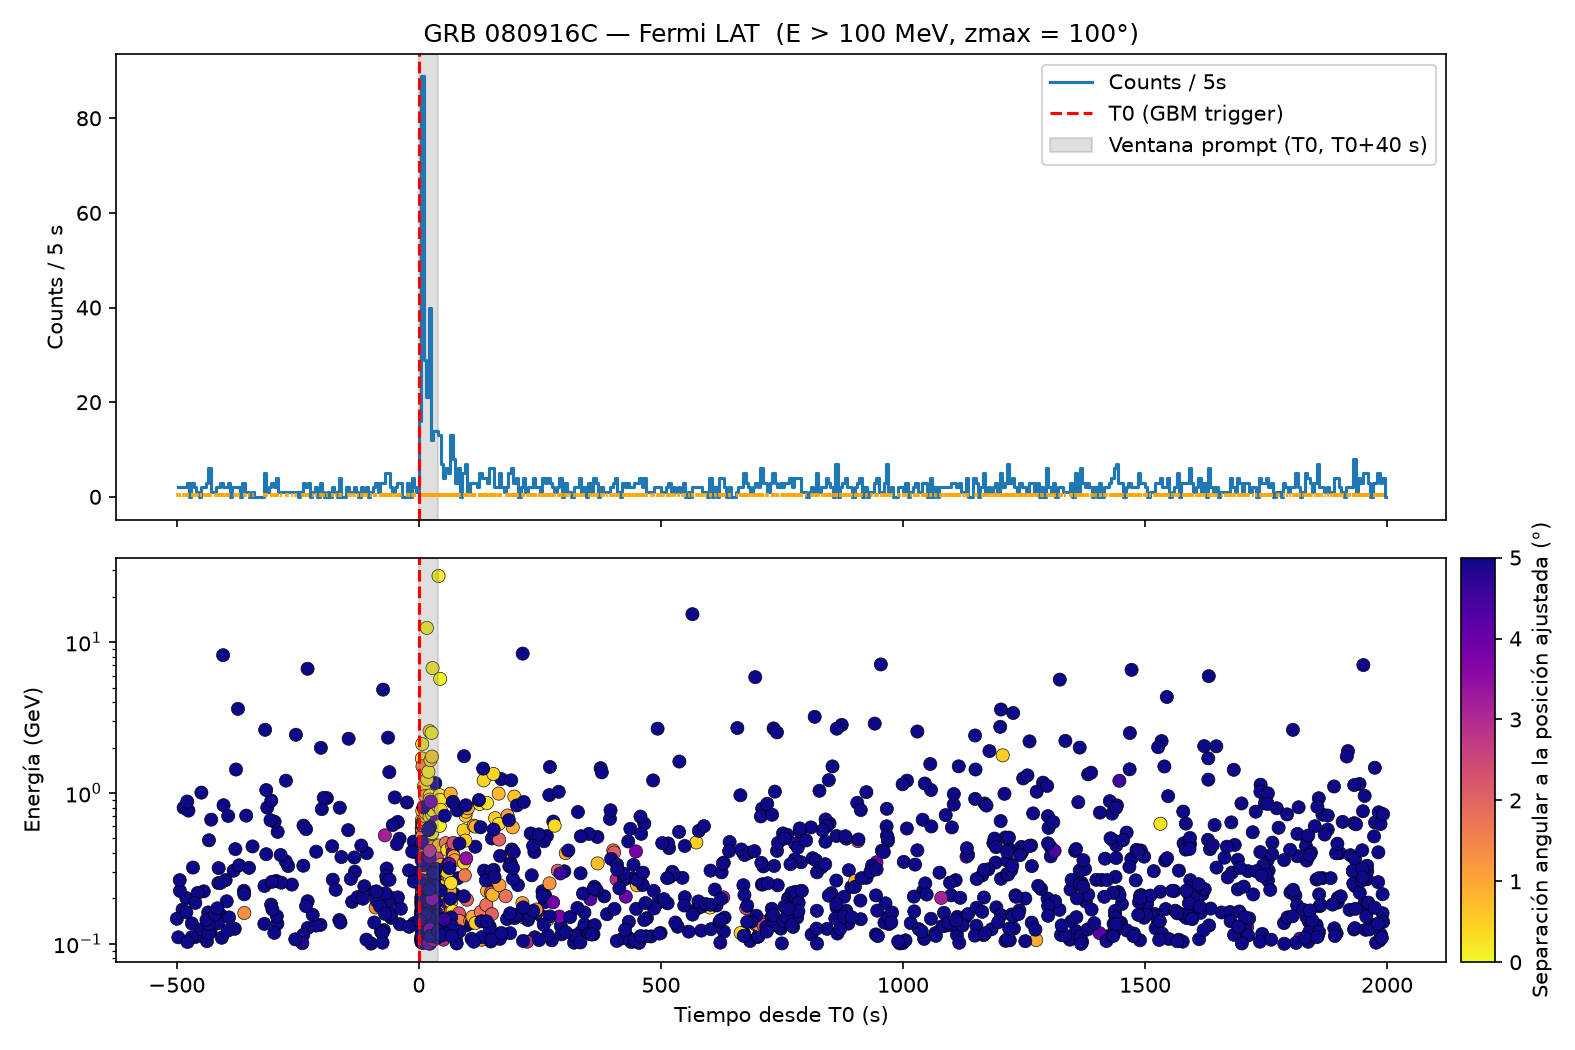
\includegraphics[width=0.95\textwidth]{PNGs/LC_080916C.png}
    \caption{Curva de luz del GRB 080916C en la banda del LAT ($E>100$~MeV, corte \texttt{zmax} $=100^{\circ}$).
    El panel superior muestra los conteos en bins de 5~s, con una marca naranja por cada fotón y la ventana
    de la fase prompt ($T_0$ a $T_0+40$~s) sombreada en gris. El panel inferior muestra la energía de cada
    fotón contra su tiempo de llegada, con el color indicando la separación angular respecto a la posición
    ajustada: los fotones más cercanos a la fuente (colores claros) se concentran en la ventana prompt,
    donde el estallido domina por completo la región.}
    \label{fig:lc080916C}
\end{figure}

La fase prompt ($T_0$ a $T_0+40$~s) dejó 219 conteos en 37~s de exposición viva, suficientes para el
análisis \textit{binned}. El ajuste en XSPEC de una ley de potencia simple con el estadístico de Cash dio
un índice fotónico $\mathrm{PhoIndex} = 2.32 \pm 0.08$, con C-stat $=26.4$ para 28 grados de libertad
(un ajuste bueno: del orden de una unidad de estadístico por grado de libertad), del orden de los valores
reportados para la emisión de alta energía de este evento \cite{Ackermann2013}. La Figura~\ref{fig:xspec080916C}
muestra el espectro ajustado y sus residuos normalizados.

\begin{figure}[h!]
    \centering
    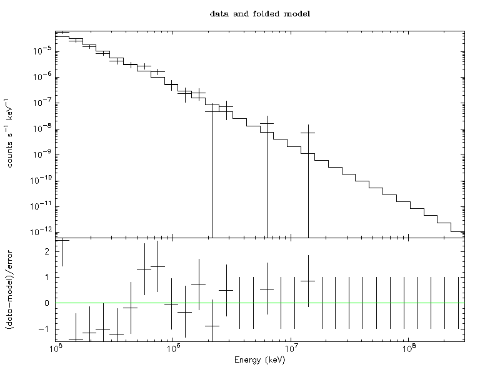
\includegraphics[width=0.75\textwidth]{PNGs/XSPEC_080916C_fit.png}
    \caption{Ajuste espectral en XSPEC de la fase prompt del GRB 080916C (modelo \texttt{powerlaw},
    estadístico de Cash). Arriba, el espectro de conteos observado y el modelo convuelto con la respuesta
    del instrumento; abajo, los residuos divididos entre la incertidumbre de cada canal, que oscilan
    alrededor de cero sin estructura: la ley de potencia simple describe bien los datos.}
    \label{fig:xspec080916C}
\end{figure}

Para la emisión extendida ($T_0+40$ a $T_0+400$~s, clase \texttt{SOURCE}) quedaron 99 fotones en la
región. El ajuste unbinned con \texttt{gtlike} dio una detección contundente:
$\mathrm{TS} = 455$ (una significancia aproximada de $\sqrt{\mathrm{TS}} \approx 21\sigma$), con índice
$\Gamma = -2.02 \pm 0.11$ y un flujo de $(6.2 \pm 0.8)\times10^{-5}$~ph~cm$^{-2}$~s$^{-1}$ entre 100~MeV
y 200~GeV. De los 99 fotones, el modelo atribuye 70.2 al GRB: incluso 40~s después del disparo, el
estallido seguía dominando la región. La Tabla~\ref{tab:resumen080916C} resume ambos ajustes y la
Figura~\ref{fig:espectro080916C} muestra el espectro de conteos con las componentes del modelo.

\begin{table}[h!]
\centering
\caption{Resumen del análisis del GRB 080916C. La fase prompt se ajustó con el método binned (XSPEC,
ley de potencia simple, estadístico de Cash) y la emisión extendida con el método unbinned
(\texttt{gtlike}). En XSPEC el índice se define positivo, $N(E)\propto E^{-\mathrm{PhoIndex}}$, de modo
que $\mathrm{PhoIndex}=2.32$ equivale a $\Gamma=-2.32$ en la convención de \texttt{gtlike}.}
\label{tab:resumen080916C}
\begin{tabular}{lcc}
\toprule
 & \textbf{Prompt (binned)} & \textbf{Extendida (unbinned)} \\
\midrule
Ventana & $T_0$ a $T_0+40$~s & $T_0+40$ a $T_0+400$~s \\
Clase de eventos & \texttt{TRANSIENT} & \texttt{SOURCE} \\
Fotones en la región & 219 & 99 \\
Índice & $\mathrm{PhoIndex} = 2.32 \pm 0.08$ & $\Gamma = -2.02 \pm 0.11$ \\
Flujo [ph~cm$^{-2}$~s$^{-1}$] & --- & $(6.2 \pm 0.8)\times10^{-5}$ \\
Bondad / detección & C-stat $= 26.4/28$ g.l. & $\mathrm{TS} = 455$ ($\approx 21\sigma$) \\
Npred (GRB) & --- & 70.2 \\
\bottomrule
\end{tabular}
\end{table}

\begin{figure}[h!]
    \centering
    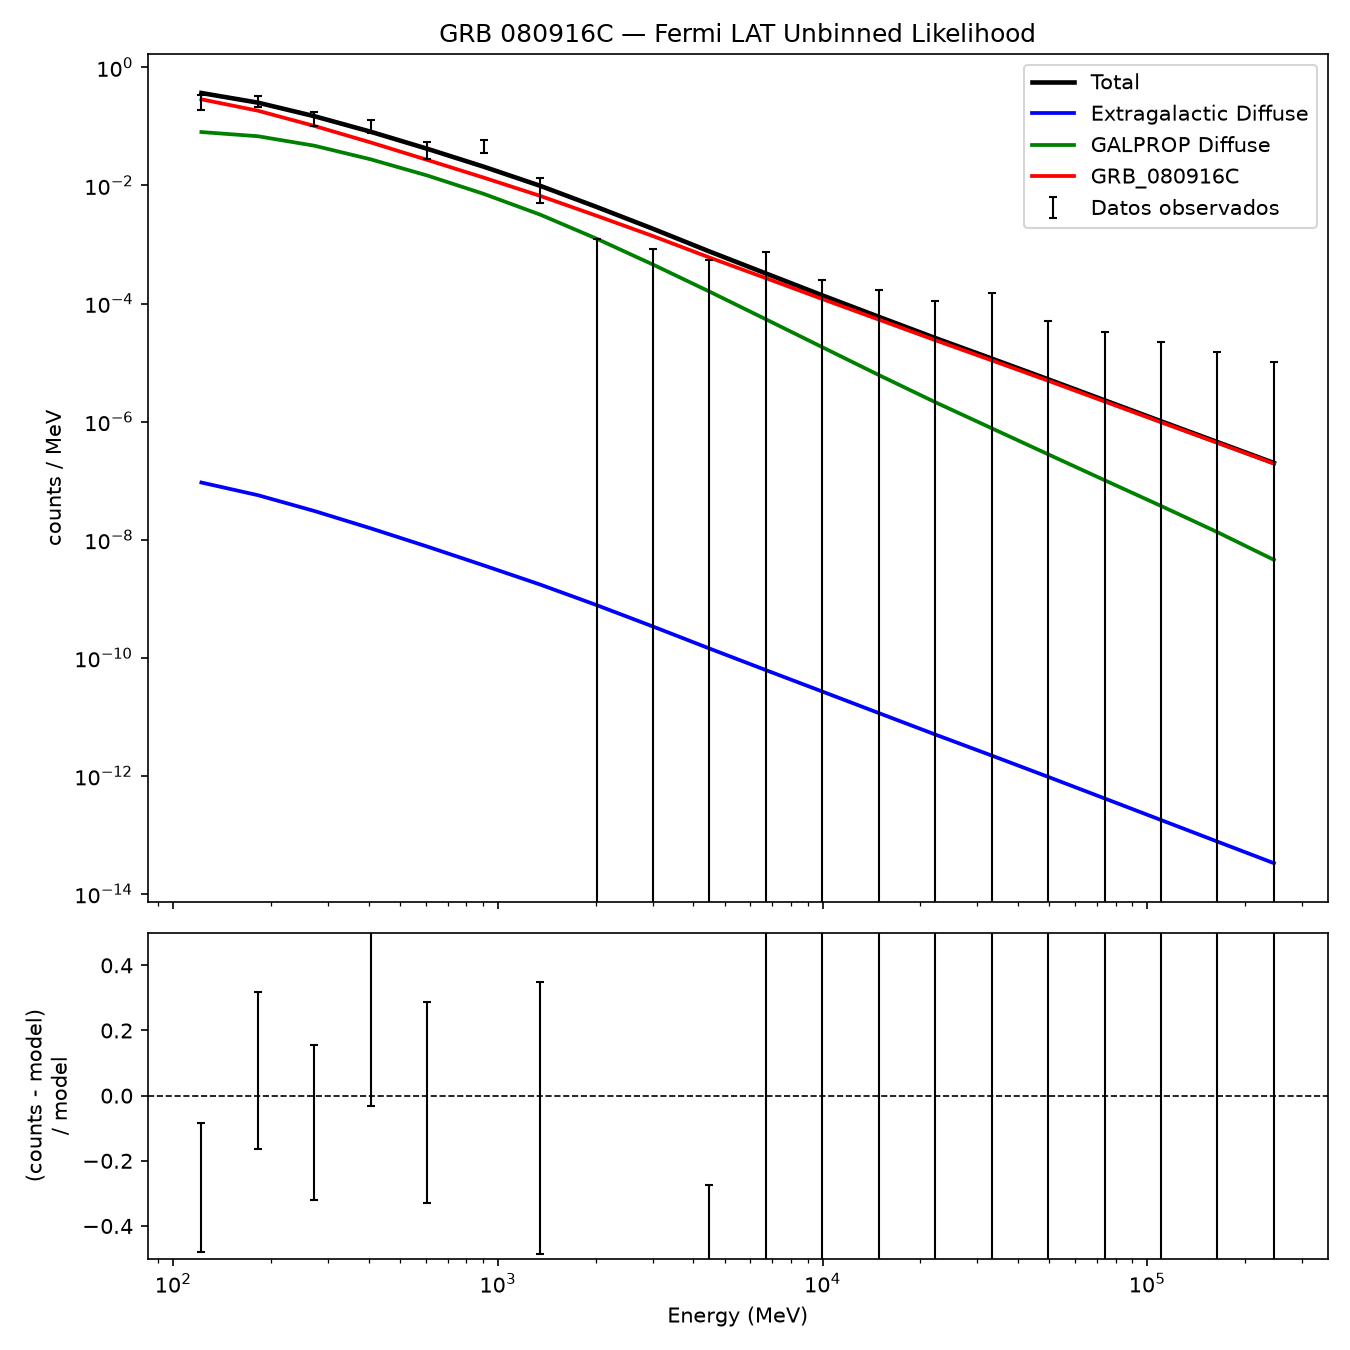
\includegraphics[width=0.8\textwidth]{PNGs/Espectro_080916C.png}
    \caption{Espectro de conteos de la emisión extendida del GRB 080916C y componentes del modelo
    ajustado con \texttt{gtlike}: en rojo la fuente puntual del GRB, en verde el difuso galáctico
    (GALPROP), en azul el difuso extragaláctico y en negro la suma, con los datos y sus barras de error
    poissonianas. El panel inferior muestra los residuos relativos (conteos $-$ modelo)/modelo. El GRB
    domina sobre los fondos en prácticamente toda la banda, como corresponde a un evento tan brillante.}
    \label{fig:espectro080916C}
\end{figure}

Un detalle del ajuste merece mención honesta: con una ventana tan corta, las dos componentes difusas del
modelo son casi degeneradas entre sí, y el ajuste llevó el prefactor del fondo isotrópico a su cota
inferior (Npred $\approx 0$) mientras la normalización galáctica subía a $2.10 \pm 0.42$. Para el
propósito de esta validación eso es inocuo —los fondos enteros aportan $\sim$29 de los 99 fotones y el
GRB está detectado a $21\sigma$ se reparta como se reparta el difuso—, pero anticipa el problema que
domina el siguiente análisis: cuando los fotones escasean, el reparto entre fuente y fondos se vuelve la
decisión central.

\subsection{GRB 251118A}

\subsubsection{Datos, posición y selección de eventos}

El GRB 251118A fue detectado por el GBM el 18 de noviembre de 2025 a las 20:31:30.09 UT
($T_0 = 785190695.09$~s MET), con $T_{90} = 46.6$~s en la banda de 50--300~keV y una fluencia de
$(1.03\pm0.01)\times10^{-4}$~erg~cm$^{-2}$ \cite{GCN42783}: en rayos gamma de baja energía fue un
estallido brillante. El LAT lo detectó y localizó en RA $=160.08^{\circ}$, Dec $=-34.58^{\circ}$
($\pm0.17^{\circ}$, 90\,\% de contención) \cite{GCN42752}, pero en condiciones adversas: al momento del
disparo la fuente estaba a $69^{\circ}$ del eje óptico del instrumento (el \textit{boresight}, la normal
al plano superior del LAT, desde donde se mide el ángulo de incidencia), casi al borde del campo de
visión útil ($\sim$70$^{\circ}$), donde el área efectiva es mínima. Eso explica que, siendo brillante en
keV, en el LAT dejara apenas unas decenas de fotones.

El seguimiento de Swift encontró el afterglow del estallido: XRT lo detectó en rayos X decayendo como
$t^{-1.08}$ \cite{GCN42782} y UVOT midió su contraparte óptica en RA $=160.00422^{\circ}$,
Dec $=-34.52254^{\circ}$ con una precisión de $0.42''$ \cite{GCN42786}, a $5'$ de la posición del LAT y
dentro de su radio de error. Esa posición de UVOT, cuya incertidumbre es despreciable frente a la PSF
del LAT, es la que se adoptó para la fuente puntual y para todas las separaciones angulares; con ella,
el paso de localización con \texttt{gtfindsrc} resulta innecesario.

Los datos se solicitaron en un cono de 30$^{\circ}$ alrededor de la posición del LAT, de $T_0-1000$ a
$T_0+3700$~s y entre 100~MeV y 300~GeV (700 eventos en la consulta). Sobre ellos se hicieron dos
selecciones con la clase \texttt{SOURCE} y \texttt{zmax} $=100^{\circ}$, ambas con radio de
15$^{\circ}$: una \textbf{ventana de análisis} de $T_0$ a $T_0+1500$~s —la misma que usa la circular del
LAT para el flujo, de modo que ambos resultados sean directamente comparables—, que tras
\texttt{gtmktime} quedó con \textbf{35 fotones} en un único intervalo de buen tiempo de 1500~s, y una
\textbf{ventana larga} de $T_0-100$ a $T_0+3600$~s, solo para la curva de luz, con 39 fotones en 2512~s
de buen tiempo. La Tabla~\ref{tab:radios251118A} muestra cómo se reparten los fotones de la ventana de
análisis según la distancia a la posición del GRB.

\begin{table}[h!]
\centering
\caption{Fotones de la ventana de análisis del GRB 251118A ($T_0$ a $T_0+1500$~s, clase \texttt{SOURCE},
\texttt{zmax} $=100^{\circ}$) según el radio de extracción medido desde la posición del afterglow de
UVOT. La concentración hacia radios pequeños —5 fotones dentro de $1^{\circ}$— ya sugiere una fuente
puntual sobre un fondo repartido por toda la región.}
\label{tab:radios251118A}
\begin{tabular}{lc}
\toprule
\textbf{Radio de extracción} & \textbf{Fotones} \\
\midrule
$< 15^{\circ}$ & 35 \\
$< 10^{\circ}$ & 18 \\
$< 5^{\circ}$  & 9 \\
$< 2^{\circ}$  & 5 \\
$< 1^{\circ}$  & 5 \\
$< 0.5^{\circ}$ & 3 \\
\bottomrule
\end{tabular}
\end{table}

\subsubsection{Curva de luz y nivel de fondo}

La Figura~\ref{fig:lc251118A} muestra la curva de luz de la ventana larga en bins de 50~s, junto con la
energía y la separación angular de cada fotón. Los cinco fotones que llegaron a menos de 1$^{\circ}$ de
la posición del afterglow lo hicieron a los 279, 578, 1239, 1394 y 1457~s después del disparo, mucho
después de que terminara la emisión prompt registrada por el GBM, cuyo $T_{90}$ de 46.6~s aparece como
una banda gris en la figura. La emisión que detectó el LAT no corresponde entonces a la cola del
estallido en keV, sino a una fase posterior. El aumento de conteos que se observa entre $\sim$400 y
$\sim$700~s se debe, en cambio, a fotones que llegaron lejos de la posición del GRB y que corresponden
en su mayoría al fondo.

Entre esos cinco fotones está el de mayor energía de la ventana, de 6.8~GeV, que llegó a
$T_0+1394$~s y se reconstruyó a solo 0.05$^{\circ}$ de la posición del afterglow. Se trata del mismo
fotón que reporta la circular del LAT \cite{GCN42752}, y su cercanía a esa posición es la indicación más
directa, previa a cualquier ajuste, de que los datos contienen emisión del GRB.

Después de $\sim$1500~s no llegó ningún fotón a la región. Entre $T_0+2000$ y $T_0+3600$~s el
instrumento acumuló solo 412~s de buen tiempo, porque el barrido del cielo sacó la región del campo de
visión, de modo que la ausencia de fotones en ese intervalo es consistente con el apagado de la fuente,
pero no alcanza para medir la tasa de fondo. Por esa razón, el fondo se estima con el modelo del ajuste
de máxima verosimilitud que se presenta en las secciones siguientes.

\begin{figure}[h!]
    \centering
    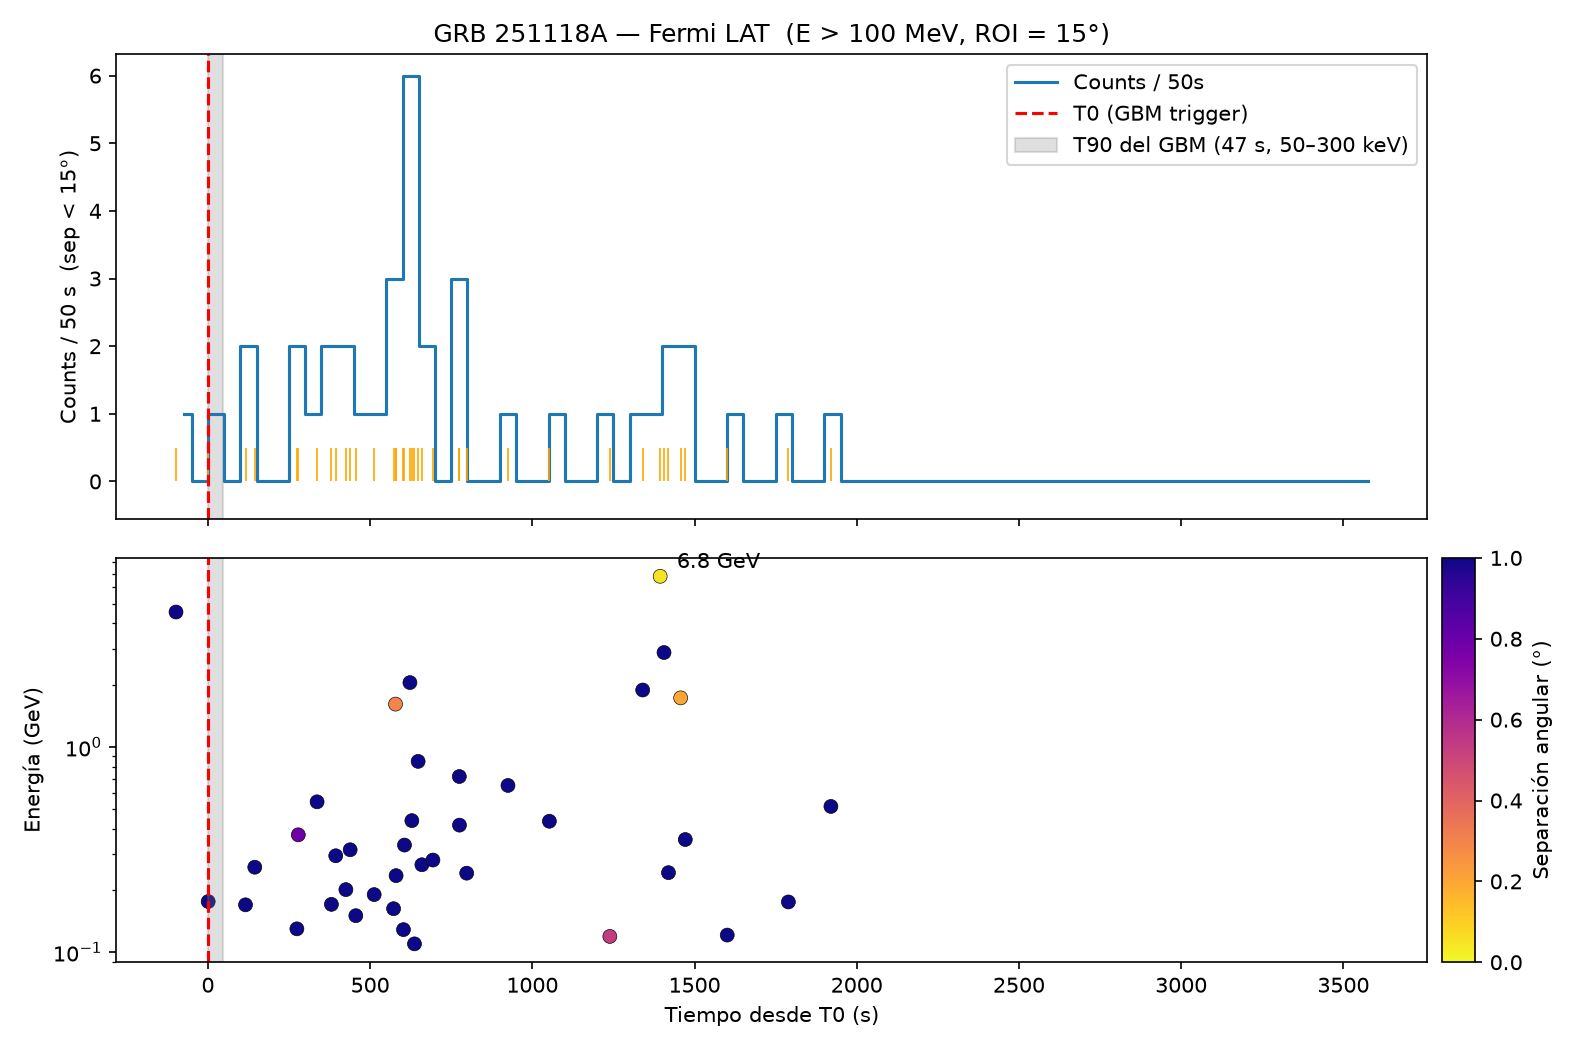
\includegraphics[width=0.95\textwidth]{PNGs/LC_251118A_larga.png}
    \caption{Curva de luz del GRB 251118A en la banda del LAT ($E>100$~MeV, radio de 15$^{\circ}$),
    de $T_0-100$ a $T_0+3600$~s. El panel superior muestra los conteos en bins de 50~s y una marca
    naranja por cada fotón, y la banda gris corresponde al $T_{90}$ del GBM (46.6~s, 50--300~keV). El
    panel inferior muestra la energía de cada fotón contra su tiempo de llegada, y el color indica su
    separación angular respecto a la posición del afterglow, desde amarillo (sobre la fuente) hasta azul
    oscuro (1$^{\circ}$ o más). El fotón de 6.8~GeV, que llegó a $T_0+1394$~s, aparece prácticamente
    sobre la posición del afterglow.}
    \label{fig:lc251118A}
\end{figure}

\subsubsection{Modelo de la región y variantes del ajuste}

El modelo de la región tiene las tres componentes descritas en la Metodología, que son la fuente puntual
del GRB en la posición del afterglow, con un espectro de ley de potencia (\texttt{PowerLaw2}), el difuso
galáctico (GALPROP) y el fondo isotrópico. El prefactor y el índice del fondo isotrópico se dejaron fijos
en sus valores de catálogo, porque con 35 fotones el ajuste se vuelve inestable cuando todas las
normalizaciones quedan libres y la matriz de covarianza deja de ser definida positiva.

El GRB se encuentra a una latitud galáctica de $b = 21^{\circ}$ y la región de interés tiene un radio de
15$^{\circ}$, por lo que el plano galáctico queda fuera de ella y la contribución galáctica proviene de
la emisión difusa a latitudes medias. El modelo tampoco incluye las fuentes puntuales del catálogo 4FGL
que hay dentro de la región. Su aporte en 1500~s es muy pequeño comparado con el de los fondos difusos,
pero su omisión es una limitación de este análisis.

Cuando hay tan pocos fotones, la decisión de modelado que más influye en el resultado es cuáles
parámetros se fijan y cuáles se dejan libres. Para examinarla se ajustaron cuatro variantes del mismo
modelo sobre los mismos datos, descritas en la Tabla~\ref{tab:variantes251118A}, y cada par de variantes
difiere en una sola decisión. La comparación entre V1 y V2 muestra el efecto de fijar la normalización
galáctica en su valor nominal de 1. La comparación entre V2 y V3 muestra el efecto de fijar además el
índice del GRB en el valor de la circular ($-1.8$), algo que solo es posible porque este GRB ya cuenta con
una circular y que no podría hacerse con un evento nuevo. Por último, la comparación entre V4 y V1 sirve
como control, ya que \texttt{PowerLaw} y \texttt{PowerLaw2} son la misma ley de potencia escrita de dos
maneras y deberían dar el mismo resultado.

\begin{table}[h!]
\centering
\caption{Las cuatro variantes del modelo ajustadas al GRB 251118A. La columna ``Espectro GRB'' indica cuál de
las dos formas de la ley de potencia descritas en la Metodología se usó para la fuente puntual. La
última columna enumera los parámetros que quedaron libres en todo el modelo, incluida la normalización
galáctica cuando no está fija.}
\label{tab:variantes251118A}
\small
\setlength{\tabcolsep}{4.5pt}
\begin{tabular}{lllll}
\toprule
\textbf{Variante} & \textbf{Índice GRB} & \textbf{GALPROP} & \textbf{Espectro GRB} & \textbf{Parámetros libres} \\
\midrule
V1 & libre & libre & \texttt{PowerLaw2} & Integral, Index, Value (3) \\
V2 & libre & fija $=1$ & \texttt{PowerLaw2} & Integral, Index (2) \\
V3 & fijo $=-1.8$ & fija $=1$ & \texttt{PowerLaw2} & Integral (1) \\
V4 & libre & libre & \texttt{PowerLaw} & Prefactor, Index, Value (3) \\
\bottomrule
\end{tabular}
\end{table}

\subsubsection{Ajuste de máxima verosimilitud}

La Tabla~\ref{tab:gtlike251118A} presenta los resultados de las cuatro variantes. Como las variantes
tienen distinto número de parámetros libres, sus valores de TS no se comparan directamente. La
significancia de cada una se calculó a partir de su TS y del número de parámetros libres que corresponden
al GRB, que son dos en V1, V2 y V4 (el flujo y el índice) y uno en V3 (solo el flujo). Solo en este último
caso la significancia coincide con $\sqrt{\mathrm{TS}}$.

\begin{table}[h!]
\centering
\caption{Resultados del ajuste unbinned del GRB 251118A para las cuatro variantes del modelo
(ventana $T_0$ a $T_0+1500$~s, radio de 15$^{\circ}$). Se reportan el número de parámetros libres de todo
el modelo, el TS con su significancia aproximada (calculada con los parámetros libres del GRB), el índice
y el flujo del GRB con sus errores a 1$\sigma$, el número de fotones que el modelo atribuye al GRB
(Npred) y la normalización ajustada del difuso galáctico. El isotrópico quedó fijo en sus valores de
catálogo en todas las variantes y aporta Npred $=9.4$.}
\label{tab:gtlike251118A}
\small
\setlength{\tabcolsep}{4.5pt}
\begin{tabular}{lcccccc}
\toprule
\textbf{Var.} & \textbf{Parám.} & \textbf{TS} ($\approx\sigma$) & \textbf{Índice} ($\Gamma$) & \textbf{Flujo [$10^{-6}$~ph~cm$^{-2}$~s$^{-1}$]} & \textbf{Npred} & \textbf{GALPROP} \\
\midrule
V1 & 3 & 42.7 (6.2$\sigma$) & $-1.77 \pm 0.30$ & $2.08 \pm 1.02$ & 7.4 & $1.26 \pm 0.34$ \\
V2 & 2 & 46.0 (6.5$\sigma$) & $-1.80 \pm 0.30$ & $2.22 \pm 1.03$ & 7.8 & 1 (fija) \\
V3 & 1 & 46.0 (6.8$\sigma$) & $-1.8$ (fijo) & $2.22 \pm 0.90$ & 7.8 & 1 (fija) \\
V4 & 3 & 42.7 (6.2$\sigma$) & $-1.77 \pm 0.30$ & $2.08 \pm 2.29$ & 7.4 & $1.26 \pm 0.34$ \\
\bottomrule
\end{tabular}
\end{table}

Al fijar la normalización galáctica en 1 (de V1 a V2), el TS sube de 42.7 a 46.0 y el índice queda
prácticamente en el valor de la circular. Cuando la normalización se deja libre, como en V1, converge a
$1.26 \pm 0.34$. Ese valor es compatible con 1 dentro de su error, pero tiende a crecer porque absorbe
fotones que de otro modo se atribuirían al GRB, de modo que con esta cantidad de fotones conviene fijarla
en su valor nominal.

Fijar además el índice del GRB (de V2 a V3) no cambia el TS, que se mantiene en 46.0, y su único efecto
es reducir el error del flujo de 1.03 a 0.90 ($\times10^{-6}$~ph~cm$^{-2}$~s$^{-1}$). Esa reducción es
la que se espera al quitar un parámetro libre y no representa una mejora física del ajuste. La variante
V4, por su parte, reproduce el TS y el índice de V1, lo que confirma que el cambio de parametrización no
altera el resultado. La diferencia en el error del flujo de V4 se debe a que en esa parametrización el
flujo no es un parámetro del ajuste, y su error se propaga desde el prefactor, que está fuertemente
correlacionado con el índice.

Por estas razones se adopta V2 como resultado del análisis, ya que mide el índice con los datos propios
en lugar de tomarlo de la circular y mantiene el fondo galáctico en su valor nominal. Con esta variante
se obtiene $\mathrm{TS} = 46.0$, que con dos parámetros libres del GRB equivale a unas 6.5$\sigma$, un
índice $\Gamma = -1.80 \pm 0.30$ y un flujo de $(2.22 \pm 1.03)\times10^{-6}$~ph~cm$^{-2}$~s$^{-1}$ por
encima de 100~MeV.

El mismo ajuste permite estimar cuánto fondo hay en la región. De los 35 fotones observados, el modelo
atribuye 16.1 al difuso galáctico, 9.4 al isotrópico y 7.8 al GRB, para un total predicho de 33.2
fotones. Cerca de tres de cada cuatro fotones de la región corresponden entonces al fondo, y la señal del
GRB se reduce a unos ocho fotones, lo que explica buena parte de la dificultad de este análisis. La
Figura~\ref{fig:espectro251118A} muestra el espectro de conteos con este reparto entre componentes.

\begin{figure}[h!]
    \centering
    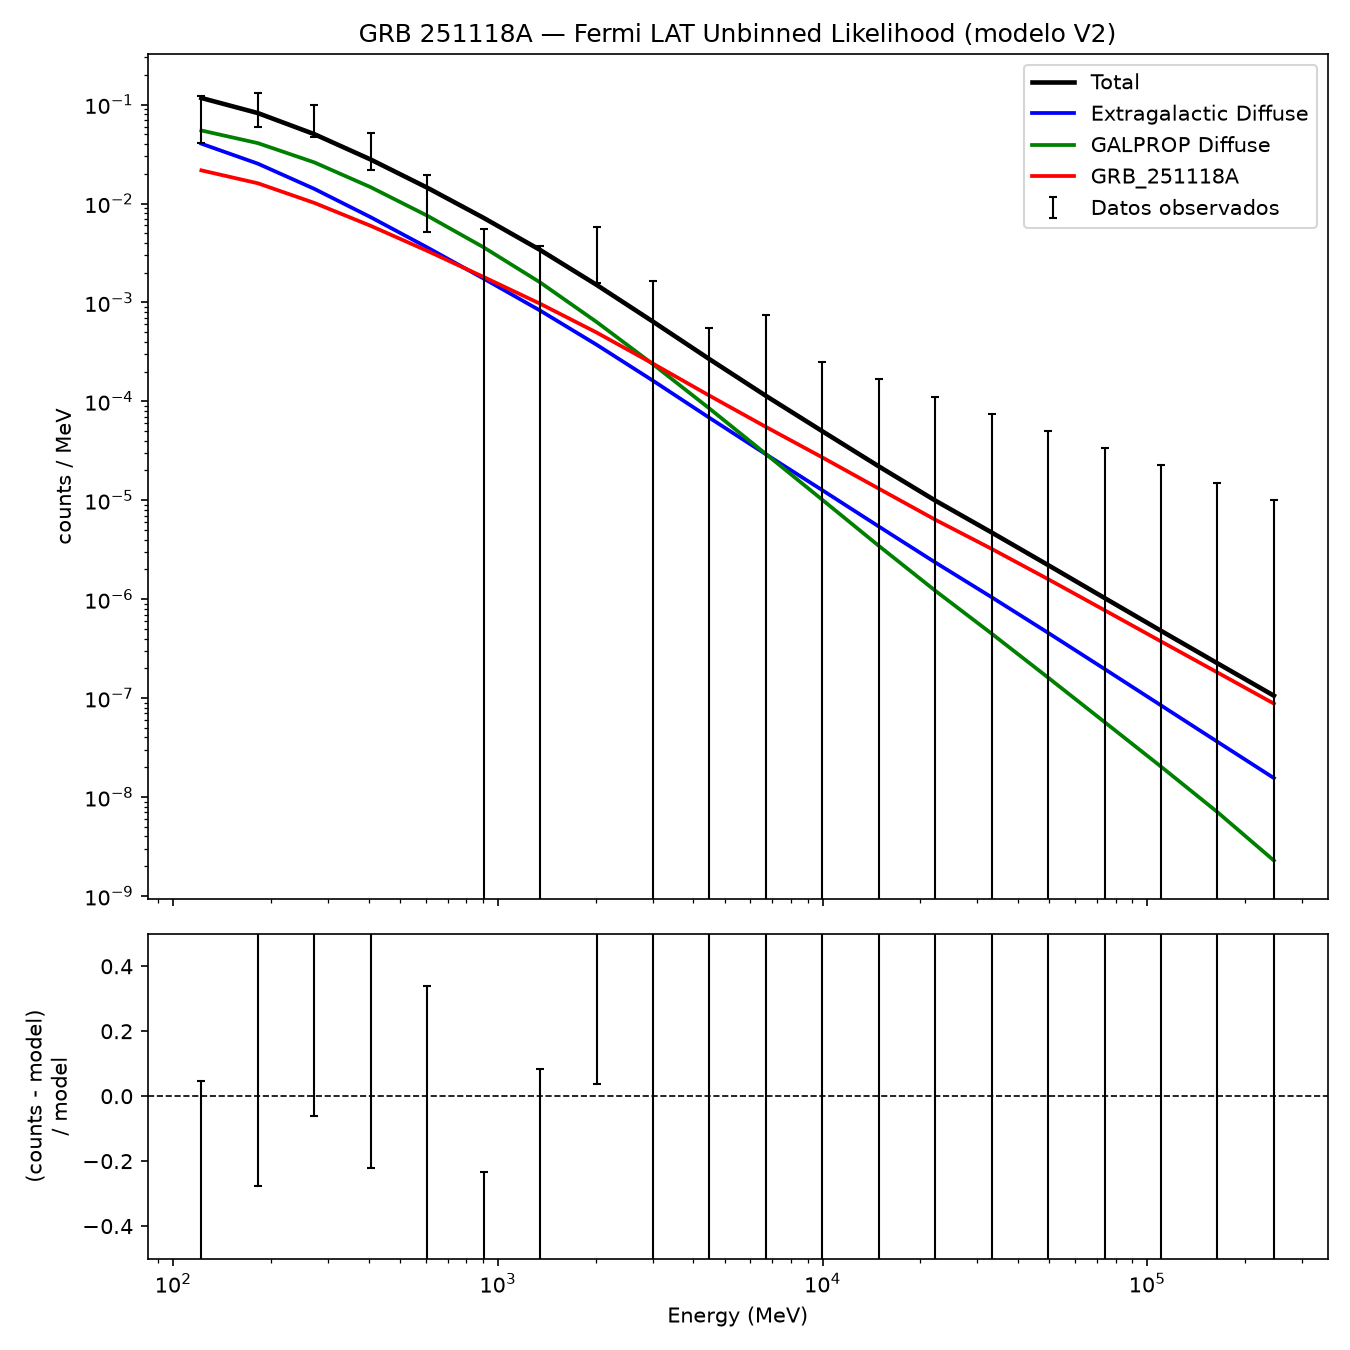
\includegraphics[width=0.82\textwidth]{PNGs/Espectro_251118A_V2.png}
    \caption{Espectro de conteos del GRB 251118A y componentes del modelo V2 ajustado con
    \texttt{gtlike}. El GRB aparece en rojo, el difuso galáctico (GALPROP) en verde, el isotrópico en
    azul y la suma en negro, junto con los datos y sus barras de error poissonianas, y el panel inferior
    muestra los residuos relativos. Por debajo de $\sim$1~GeV dominan los fondos difusos, que concentran
    la mayoría de los 35 fotones. Entre 1 y 2~GeV el GRB se vuelve comparable al fondo galáctico, y por
    encima de unos pocos GeV domina la región, por lo que el fotón de 6.8~GeV tiene un peso grande en la
    detección.}
    \label{fig:espectro251118A}
\end{figure}

\subsubsection{Verificación con el análisis binned}

Como control independiente se construyó también el espectro binned de la misma ventana, con 30 canales
logarítmicos en energía, y se ajustó en XSPEC una ley de potencia simple con el estadístico de Cash. El
ajuste dio $\mathrm{PhoIndex} = 1.98 \pm 0.17$, con un C-stat de 13.2 para 28 grados de libertad
(Figura~\ref{fig:xspec251118A}).

Este control tiene una limitación importante. El ajuste binned no incluye un modelo de fondo, por lo que
su ley de potencia describe el total de fotones de la región, es decir, el GRB junto con los cerca de 25
fotones de los fondos difusos, y no al GRB por separado. Por eso, que su índice quede a 0.5$\sigma$ del
índice del GRB obtenido en el ajuste unbinned indica únicamente que la forma espectral del conjunto es
coherente con la del GRB. La medición del GRB propiamente dicha es la del ajuste unbinned.

XSPEC reporta además, junto al ajuste, una probabilidad nula que se calcula con la estadística
$\chi^{2}$. Ese valor no es interpretable en este caso, porque con 35 fotones repartidos en 30 canales la
mayoría de los canales tiene 0, 1 o 2 conteos y la estadística $\chi^{2}$ deja de ser válida. Por esa
razón, la bondad del ajuste se evalúa con el C-stat en relación con sus grados de libertad.

\begin{figure}[h!]
    \centering
    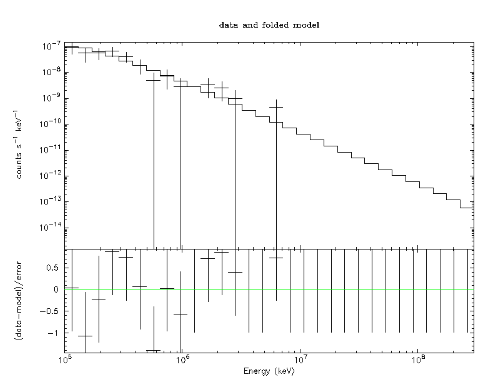
\includegraphics[width=0.75\textwidth]{PNGs/XSPEC_251118A_fit.png}
    \caption{Ajuste espectral binned del GRB 251118A en XSPEC (modelo \texttt{powerlaw}, estadístico de
    Cash) sobre la ventana de análisis completa. El panel superior muestra el espectro de conteos y el
    modelo convolucionado con la respuesta del instrumento, y el inferior los residuos divididos entre la
    incertidumbre de cada canal. Las barras de error grandes corresponden a canales con 0 o 1 conteos, algo
    inevitable con 35 fotones en 30 canales. Aun así, los residuos no muestran una estructura sistemática y
    la ley de potencia describe bien el conjunto.}
    \label{fig:xspec251118A}
\end{figure}

\subsubsection{Comparación con la circular GCN y lectura física}

Para decidir si dos mediciones coinciden no basta con comparar sus valores centrales. Es necesario
dividir su diferencia entre la incertidumbre combinada, $|x_1-x_2|/\sqrt{\sigma_1^{2}+\sigma_2^{2}}$, y
se considera que dos valores son consistentes cuando el resultado es menor que 2. La
Tabla~\ref{tab:comparacion251118A} aplica este criterio a los resultados de este trabajo y a los de la
circular del LAT \cite{GCN42752}. Conviene tener presente que ambas mediciones se hicieron con los mismos
fotones, de manera que no son independientes y la incertidumbre combinada sirve solo como una medida
orientativa del acuerdo.

\begin{table}[h!]
\centering
\caption{Comparación de los resultados del GRB 251118A con la circular GCN 42752, en unidades de la
incertidumbre combinada ($\sigma$ comb.). El índice de XSPEC se expresa en la convención de
\texttt{gtlike} ($\Gamma = -\mathrm{PhoIndex}$). Su flujo no se reporta porque la normalización de XSPEC
no es directamente un flujo de fotones y, al no haber modelo de fondo, correspondería al total de la
región.}
\label{tab:comparacion251118A}
\small
\setlength{\tabcolsep}{4.5pt}
\begin{tabular}{lcccc}
\toprule
\textbf{Análisis} & \textbf{Índice} ($\Gamma$) & $\sigma$ \textbf{comb.} & \textbf{Flujo [$10^{-6}$~ph~cm$^{-2}$~s$^{-1}$]} & $\sigma$ \textbf{comb.} \\
\midrule
Unbinned, V2 (este trabajo) & $-1.80 \pm 0.30$ & 0.0 & $2.22 \pm 1.03$ & 0.3 \\
Binned, XSPEC (este trabajo) & $-1.98 \pm 0.17$ & 0.5 & --- & --- \\
GCN 42752 & $-1.8 \pm 0.3$ & --- & $1.8 \pm 0.7$ & --- \\
\bottomrule
\end{tabular}
\end{table}

El índice obtenido coincide con el de la circular, con una diferencia de 0.0$\sigma$, y el flujo difiere
en 0.3$\sigma$. El valor central del flujo es ligeramente mayor que el de la circular, una diferencia que
cabe dentro de la fluctuación de Poisson que se espera cuando la señal es de unos ocho fotones. El
control binned queda a 0.5$\sigma$ de ambos índices. Hay que considerar que la circular proviene del
análisis automático de la colaboración, calibrado con cientos de GRB, por lo que el hecho de que este
análisis manual la reproduzca valida el flujo de trabajo aprendido, que era el objetivo de la práctica.

En cuanto a la interpretación física, la emisión prompt registrada por el GBM terminó en unos 47~s y su
espectro, descrito por una función de Band, tiene en la parte de alta energía un índice
$\beta = -2.56 \pm 0.06$ \cite{GCN42783}. El LAT, en cambio, registró fotones hasta unos 1500~s después
del disparo, con un índice $\Gamma = -1.80 \pm 0.30$, es decir, un espectro más duro que la cola de alta
energía del prompt, con una diferencia de 2.5$\sigma$ combinadas. La llegada tardía de los fotones y su
espectro más duro apuntan a que la emisión GeV del GRB 251118A no es una extrapolación del prompt, sino
una componente distinta y posterior, consistente con el afterglow temprano que Swift-XRT observó decaer
como $t^{-1.08}$ \cite{GCN42782}. Como no se ha reportado un corrimiento al rojo para este evento, no es
posible convertir estos flujos en energía isotrópica.
